A point query is a database operation that finds the records that exactly match our query conditions. In this project, we perform point query on $1$-dimensional data and $2$ dimensional data. We assign the database records into pages, predict the page index with the index models and then perform sequential search on the predicted page. In order to evaluate the errors that different index models are making, we focus on predicting the page indices and ignore the sequential search operation on a specific page. 

\begin{mscexample}
For example, assume we have an $1$-dimensional array $[1,2,3,4]$ and two pages such that $[1,2]\in P_0$ and $[3,4]\in P_1$. A point query for $x=2$ is expected to return 0 as the page index.
\end{mscexample}

\subsubsection{Point Query with B-Tree}

Point query in a B-Tree is to search the key with the exact same value of key in the tree. By searching in a Tree structure we can exploit the structure of tree to search for the key much faster. We do not have to linearly search the entire key space for the key anymore.\\
If the root node is a leaf node as well then it will simply search linearly and return an exact match of the key. If it doesn't find the key it will not return any value.\\
Since keys in B-tree are much larger in number and are usually of few levels we traverse the tree until we reach a leaf node and then search for an exact match to the point key in the leaf node. \\
To do this, firstly, we compare the point key with each key in the root node and find a key value which is greater than the point key in the root node. It will then traverse and search in the child of the key before it. We do this because we know that there is no possibility of finding the key in the child node associated with the keys which have a value higher than the Point query key. We then recursively keep traversing down the tree until we reach the desired leaf node. We then search for the key linearly in the leaf node.

\begin{mscexample}
For example if we were to search for $\mathcal{K}(\boldsymbol{x})$ $(41)$ in the example \ref{B-Tree Insertion} of the B-Tree above, we would first compare point query $(41)$ and the only $\mathcal{K}(\boldsymbol{x})$ in root node is $(11)$. Since $(11) < (31)$ and there are no keys greater than this in the root node it will search in the right child of the root node. It will then linearly search the node and since there is an exact match it will return the associated value with it.
\end{mscexample}

% TODO: This algorithm needs to be revised for B-Tree 

\begin{algorithm}[H]
    \SetAlgoLined
    \SetKwInOut{Input}{Input}
     \Input{\texttt{$\mathcal{K}(\boldsymbol{x}) ; [x \in \mathbb{R}]$, root ; Root of the B-Tree}}
    \SetKwInOut{Output}{Output}
     \Output{\texttt{Value associated with key}}
     \For{$i\gets0$ \KwTo $len(Root Node)$}{
         \If{keys in root greater than k}
         {
            \texttt{SEARCH\_CHILD($\mathcal{K}(\boldsymbol{x}, \boldsymbol{y})$)} //Search linearly the child associated with the key location one before\\
            \eIf{Child is a leaf}
            {
                \texttt{Linearly search until the $\mathcal{K}(\boldsymbol{x}, \boldsymbol{y})$ is reached}
            }
            {
                \texttt{SEARCH\_CHILD($\mathcal{K}(\boldsymbol{x}, \boldsymbol{y})$)}
            }
            
         }
    }
     \caption{Algorithm for B-Tree Search}
     \label{B-Tree Search}
\end{algorithm}

\subsubsection{Point Query with $K$D-Tree Model Index}

\begin{algorithm}[H]
    \SetAlgoLined
    \SetKwInOut{Input}{Input}
    \SetKwInOut{Output}{Output}
    \Input{\texttt{TestPoint $\mathcal{T}(\boldsymbol{x}, \boldsymbol{y}) ; [x \in \mathbb{R};y \in \mathbb{R}]$, $dim$; $2$, $split\_axis$; $0/1$ ($0$; $x\_axis$ and $1$; $y\_axis$)}}
    \Output{\texttt{Value associated with $\mathcal{T}(\boldsymbol{x}, \boldsymbol{y})$}}
    \texttt{SEARCH\_POINT\_QUERY($dim$, $split\_axis$)}\\
    \texttt{Start at root}\\
    \eIf {node is leaf}
        {
            \texttt{return value associated with node}
        }
        {
        \eIf{\texttt{$\mathcal{T}(\boldsymbol{x}, \boldsymbol{y})A$ $split\_axis$ value > node $split\_axis$ value}}
            {\texttt{Traverse to node.rightChild}\\ \texttt{SEARCH\_POINT\_QUERY($dim$, $(split\_axis+1) \% dim$)}}
        {\texttt{Traverse to node.leftChild}\\ 
        \texttt{SEARCH\_POINT\_QUERY($dim$, $(split\_axis+1) \% dim$)}}
        }
    \caption{Point Query Algorithm for $K$D-Tree}
    \label{Point_Query_Algorithm_$K$D-Tree}
\end{algorithm}

In algorithm \ref{Point_Query_Algorithm_$K$D-Tree} 

\begin{enumerate}

    \item On line $2$, start traversing the tree from the root to look for the location of $\mathcal{T}(\boldsymbol{x}, \boldsymbol{y})$. 
    
    \item On line $3$, check if the point is a leaf. If it is a leaf then we can simply return the value associated with the point.
    
    \item On line $5$, if root point is not a leaf then we make a decision weather to go left or right.
    
    \item On line $6$, we make this decision based on the $split\_axis$ value associated with the point. At the root, we start with $split\_axis$ as $0$ ($x\_axis$). 
    
    \item On line $8$ and $11$, we then recursively call the function SEARCH\_POINT\_QUERY() and update the $split\_axis$ between $0$ and $1$ alternatively as we increase levels until we reach a leaf.

\end{enumerate}



\begin{mscexample}

    \begin{minipage}[t]{\linewidth}
        \centering
        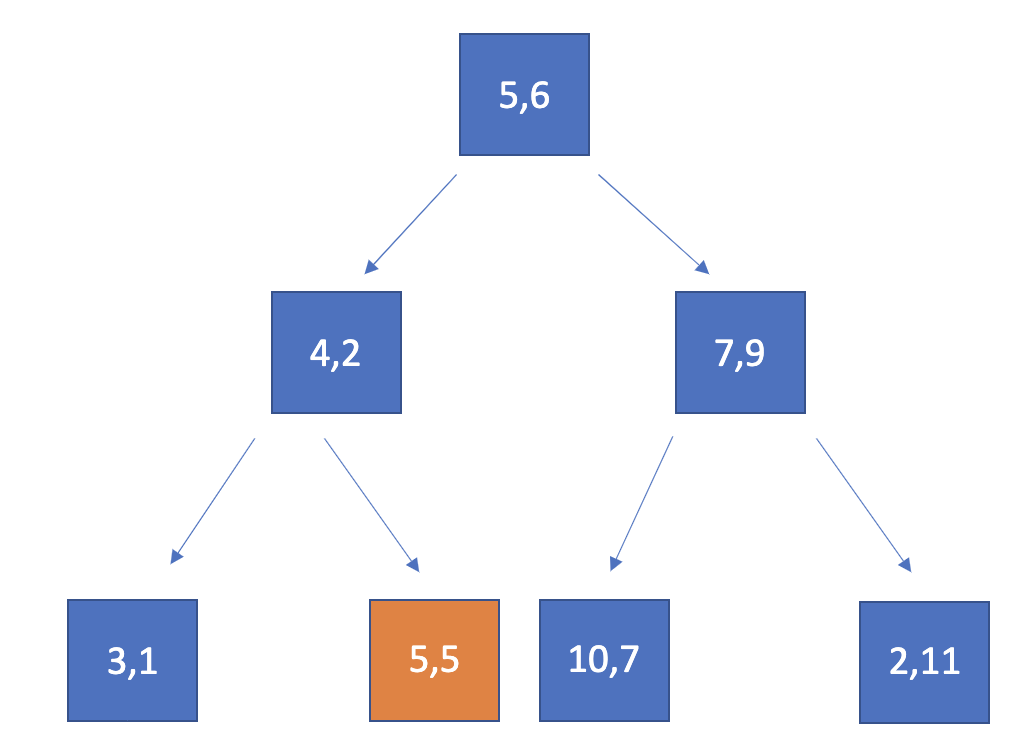
\includegraphics[width=7cm]{graphs/KD_Tree_Point_Query_Tree.png}
        % \caption{$K$D-Tree for Point Query (TestPoint $\mathcal{T}(\boldsymbol{x}, \boldsymbol{y})$ = $(5,5)$ is highlighted in orange)}
        \label{fig:$K$D-Tree_for_Point Query}
    \end{minipage}
    
    \textbf{Case 1} : For example we have a tree with Point list as 
	$$((5,6),(4,2),(7,9),(3,1),(5,5),(10,7),(2,11))$$
 Suppose we are looking for $\mathcal{T}(\boldsymbol{x}, \boldsymbol{y})$ = $(5,5)$.\\
 We start with root point $(5,6)$ and $split\_axis$ as $0$. Hence, we compare the $x\_axis$ of the $\mathcal{T}(\boldsymbol{x}, \boldsymbol{y})$ and root node. Since $5 = 5$ we move left of the root node. \\
 Next, we increase the $split\_axis$ to $1$ and so will compare the $y\_axis$ of point $(4,2)$ and  $\mathcal{T}(\boldsymbol{x}, \boldsymbol{y})$. Since $5 > 2$, we move to the right of the tree. Since node $(5,5)$ is a leaf and is the point we were searching for we return the value associated with the point. 

\end{mscexample}

\subsubsection{Point Query with Baseline Index Model}

\subsubsection{Overview}

The B-Tree can be regarded as a function $\mathcal{F}$ that maps the key $x$ into its corresponding page index $y$. It is known to us that the pages are allocated in a way that the every $S$ entries are allocated in a page where $S$ is a pre-defined parameter. For example, if we set $S$ to be 10 items per page, then the first page will contain the first 10 keys and their corresponding values. Similarly, the second 10 keys and their corresponding values will be allocated to the second page.

If we know the CDF of $X$ as $F(X\leq x)$ and the total number of entries $N$, then the position of $x$ can be estimated as $p=F(x)*N$ and the page index where it should be allocated to is given by

$$y=\floor{\frac{p}{S}}=\floor{\frac{F(x)*N}{S}}$$  

For example, if the keys are uniformly distributed from $0$ to $1000$, i.e. the CDF of $X$ is defined as $F(X\leq x)=\frac{x}{1000}$ and we set $S=10, N=1001$. Then for any key $x$, we immediately know it will be allocated into $y=\floor{\frac{1000}{10}*\frac{x}{1000}}=\floor{\frac{x}{10}}$. Assume that we have a key $698$, then we can calculate $y=\floor{\frac{698}{10}}=69$. By doing so, the page index is calculated in constant time and space.

In this example, we see that the distribution of $X$ is essential and our goal of learned index in one-dimensional data is to learn such distribution. To do so, we apply two different techniques as the baseline, the polynomial regression and fully connected neural network.

To train such a learned index, we first manually generate the $X$ with respect to a certain distribution. We then save the generated $X$ into a dense array with the length $N$. Then we use the proportional index, i.e. the index of each $x$ divided by $N$ as the expected output $y$.

\subsubsection{Polynomial Regression}
 
The polynomial regression model with degree $m$ can be formalised as 

$$ \hat{y_i}= \beta_0+\beta_1x_i+\beta_2x_i^2+\cdots+\beta_mx_i^m$$ and it can be expressed in a matrix form as below

$$
\begin{bmatrix}
y_1 \\ y_2\\ \vdots \\ y_n 
\end{bmatrix}=\begin{bmatrix}
1 & x_1 & x_1^2 &\cdots & x_1^m \\ 
1 & x_2 & x_2^2 &\cdots & x_2^m \\ 
\vdots \\ 
1 & x_n & x_n^2 &\cdots & x_n^m \\ 
\end{bmatrix}\begin{bmatrix}
\beta_0 \\ \beta_1 \\ \vdots \\ \beta_m 
\end{bmatrix}
$$ which can be written as $Y=\boldsymbol{X}\boldsymbol{\beta}$. 
 
 Our goal is to find $\beta$ such that the sum of squared error, i.e. $\text{S}(\boldsymbol{\beta})=\sum_{i=1}^n(\hat{y}-y)^2$ is minimal. This optimisation problem can be resolved by ordinary least square estimation as shown below.
 
 First we have the error as
 
 \begin{equation}
 \begin{split}
 \text{S}(\boldsymbol{\beta})=||\boldsymbol{y}-\boldsymbol{X} \boldsymbol{\beta}||& =(\boldsymbol{y}-\boldsymbol{X}\boldsymbol{\beta})^T(\boldsymbol{y}-\boldsymbol{X}\boldsymbol{\beta})\\
 	& =\boldsymbol{y}^T\boldsymbol{y}-\boldsymbol{\beta}^T\boldsymbol{X}^T\boldsymbol{y}-\boldsymbol{y}^T\boldsymbol{X}\boldsymbol{\beta}+\boldsymbol{\beta}^T\boldsymbol{X}^T\boldsymbol{X}\boldsymbol{\beta}
\end{split}
 \end{equation}
 
 Here we know that $(\boldsymbol{\beta}^T\boldsymbol{X}^T\boldsymbol{y})^T=\boldsymbol{y}^T\boldsymbol{X}\boldsymbol{\beta}$ is a $1\times 1$ matrix, i.e. a scalar. Hence it is equal to its own transpose. As a result we could simplify the error as
 
 \begin{equation}
 	\begin{split}
 		\text{S}(\boldsymbol{\beta})=\boldsymbol{y}^T\boldsymbol{y}-2\boldsymbol{\beta}^T\boldsymbol{X}^T\boldsymbol{y}+\boldsymbol{\beta}^T\boldsymbol{X}^T\boldsymbol{X}\boldsymbol{\beta}
 	\end{split}
 \end{equation}
 
 In order to find the minimum of $S(\boldsymbol{\beta})$, we differentiate it with respect to $\boldsymbol{\beta}$ as 
 
 \begin{equation}
 	\nabla_{\boldsymbol{\beta}}S=-2\boldsymbol{X}^T\boldsymbol{y}+2(\boldsymbol{X}^T\boldsymbol{X})\boldsymbol{\beta}
 \end{equation}
 
 By let it to be zero, we end up with 
 
 \begin{equation}
 \begin{split}
 	 &	-\boldsymbol{X}^T\boldsymbol{y}+(\boldsymbol{X}^T\boldsymbol{X})\boldsymbol{\beta}=0 \\
 	& \implies \boldsymbol{\beta}= (\boldsymbol{X}^T\boldsymbol{X})^{-1}\boldsymbol{X}^T\boldsymbol{y}
 \end{split}
 \end{equation}
 
\subsubsection{Fully Connected Neural Network}

\subsubsection{Point Query with Recursive Model Index}

%TODO: there should be some graph to demonstrate the last-mile problem.

In our baseline models, it is not very difficult to reduce the mean square error from millions to thousands. However, it is much harder to reduce it from thousands to tens. This is the so called last-mile problem.

In order to solve this problem, recursive model index was proposed \cite{kraska2018case}. The idea is to split the whole set of data into smaller pieces and assign each piece an index model. By doing so, each model is only responsible for a small range of keys. Ideally, in each smaller range, the keys are distributed in a way that is easier to be learned by our index models, such as polynomial model, fully connected model or even traditional B-Tree model.

As shown in Fig. \ref{rmi_structure}. A recursive model can be regarded as a tree structure, which contains a root model that receives the full dataset for training. Then the root model will split the dataset into several parts. Each sub-model will then receive one part of the full dataset. Then we train the sub-models one by one with the partial training dataset. 

\begin{mscexample}
	For example, in the Fig. \ref{rmi_structure}, the full dataset will be split into three parts and each sub-model receives one part. To train this recursive model, we first train the root model with the whole dataset. Then the root model will split the dataset into 3 parts according to the predicted value of each data point in the dataset. Then each sub-model will receive one part and we train the sub-model accordingly.
\end{mscexample}

\begin{figure*}[h]
\centering
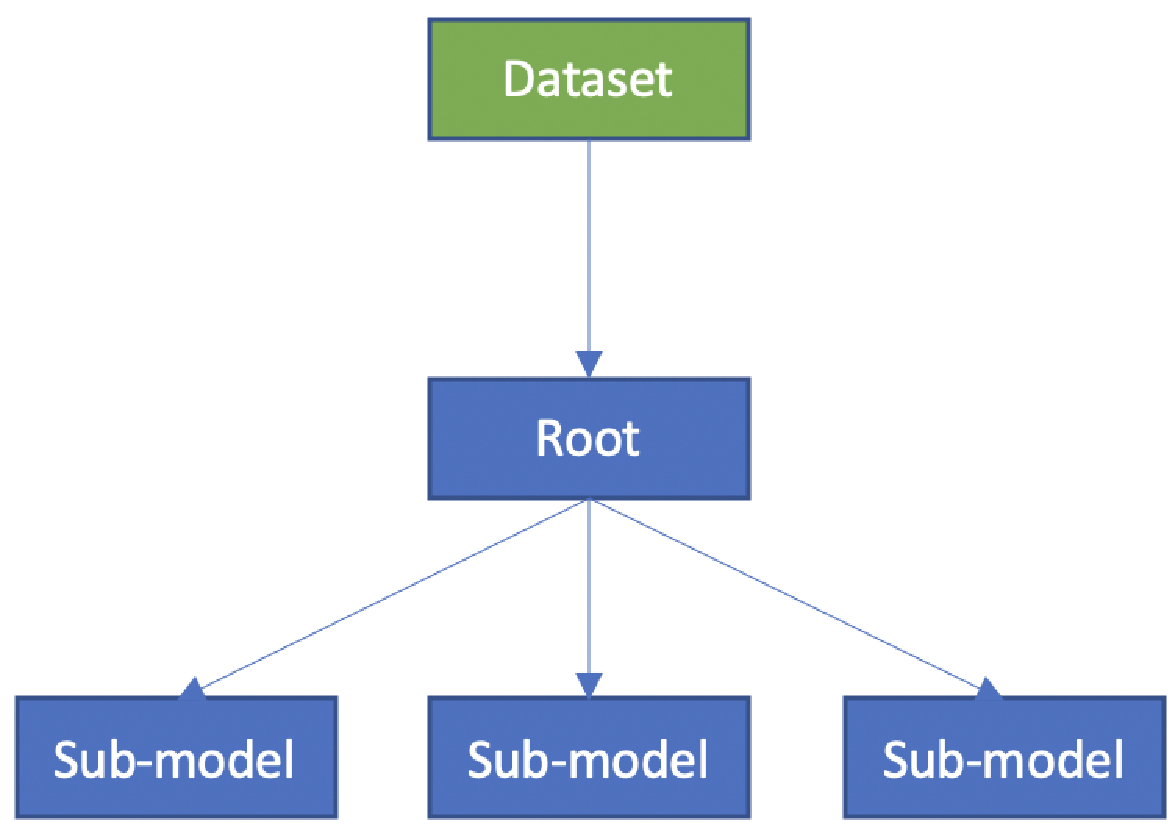
\includegraphics[scale=0.4]{graphs/rmi_demo}
\caption{An example recursive model index with one root model and three leaf model.}
\label{rmi_structure}
\end{figure*}



\subsubsection{Definitions}

Similar to a tree, we define the following terms in a recursive model:

\begin{enumerate}
	\item \textbf{Node Model}. Every node is responsible for making decisions with given input data. In one dimensional case, it can be regarded as a function $f:\mathbb{R}\to\mathbb{R}, x\to y$ where $x$ is the input index and $y$ is the corresponding page block. In principle, each node can be implemented as any machine learning model, from linear regression to neural network, or a traditional tree-based model, such as B-Tree.
	\item \textbf{Internal Node Model}. Internal nodes are all nodes except for leaf nodes and the root node. Every internal node receives a certain part of training data from the full dataset, and train a model on it. 
\end{enumerate}

In the following sections, we will use the notations defined below:
\begin{enumerate}
	\item $N_M^{(i)}$ is the number of models in the $i$th stage.
	%TODO: more notations
	%TODO: modify algorithms accordingly
\end{enumerate}


\subsubsection{Training}

In order to construct a recursive model, we need to have several parameters listed below:
\begin{enumerate}
	\item The training dataset, notated as $(X, Y)$ with entries notated as $(x,y)$.
	\item The number of stages, notated as $N_S$. It is an integer variable.
	\item The number of models at each stage, notated as $N_M$. It is a list of integer variable. $N_M^{(i+1)}$ represents the number of models in the $i$th stage.
\end{enumerate}

The training process of recursive model is an up-bottom process. There will be only one root model that receives the whole training data. After the root model is trained, we iterate over all the training data and predict the page by the root model. After the iteration, we get a new set of pairs $(X, Y_0)$. Then we map $\forall y_0\in Y_0$ into the selected model id in next stage by $\texttt{next}=y_0 * N_M^{(i+1)}/\texttt{max(Y)}$.

\begin{algorithm}[H]
    \SetAlgoLined
    \SetKwInOut{Input}{input}
    \Input{\texttt{num\_of\_stages; num\_of\_models; types\_of\_models; x; y}}
     \texttt{trainset=[[(x,y)]]} \\
     \texttt{stage$\gets 0$} \\
     \While{\texttt{stage} \textless \texttt{num\_of\_stages}}{
      \While{\texttt{model} \textless \texttt{num\_of\_models[stage]}} {
        \texttt{model.train(trainset[stage][model])} \\
        \texttt{models[stage].append(model)}
      }
      \uIf{not last stage} {
        \For{$i\gets0$ \KwTo $len(x)$}{
            	\texttt{model=models[output from previous stage]} \\
            	\texttt{output=model.predict(x[i])} \\
            	\texttt{next=output * num\_of\_models[stage+1]/max\_y} \\
            	\texttt{trainset[stage+1][next].add((x[i],y[i]))}
        }
      }
     }
     \caption{Training of Recursive Model Index}
\end{algorithm}

\subsubsection{Prediction}

\begin{algorithm}[H]
    \SetAlgoLined
    \SetKwInOut{Input}{input}
    \Input{\texttt{x; models; num\_of\_stages; max\_y}}
     \texttt{stage$\gets 0$} \\
 	 \texttt{next\_model$\gets 0$} \\
     \While{\texttt{stage} \textless \texttt{num\_of\_stages}}{
        \texttt{output = model.predict(x)} \\
        \texttt{next\_model=output*len(models[stage+1])/max\_y}\\ 
      \uIf{last stage} {
		\texttt{y = next}
      }
     }
     \caption{Training of Recursive Model Index}
\end{algorithm}

\subsubsection{Polynomial Internal Models}

In the recursive model index, we use internal models to learn the CDF of a part of the full training data. In order to learn the CDF, we need to know or assume the distribution of a specific part of the data. In this report, we support the following distributions.

\begin{table}[h]
  \begin{tabularx}{\textwidth}{@{}XX@{}}
  \toprule
    Linear Regression & $wx+b$ \\
    Quadratic Regression & $ax^2+bx+c$ \\
    B-Tree & N/A \\
    Fully Connected Neural Network & N/A \\
  \bottomrule
  \end{tabularx}
  \end{table}

Here we describe how we fit a polynomial model.

The polynomial regression model with degree $m$ can be formalised as 

$$ \hat{y_i}= \beta_0+\beta_1x_i+\beta_2x_i^2+\cdots+\beta_mx_i^m$$ and it can be expressed in a matrix form as below

$$
\begin{bmatrix}
y_1 \\ y_2\\ \vdots \\ y_n 
\end{bmatrix}=\begin{bmatrix}
1 & x_1 & x_1^2 &\cdots & x_1^m \\ 
1 & x_2 & x_2^2 &\cdots & x_2^m \\ 
\vdots \\ 
1 & x_n & x_n^2 &\cdots & x_n^m \\ 
\end{bmatrix}\begin{bmatrix}
\beta_0 \\ \beta_1 \\ \vdots \\ \beta_m 
\end{bmatrix}
$$ which can be written as $Y=\boldsymbol{X}\boldsymbol{\beta}$. 
 
 Our goal is to find $\beta$ such that the sum of squared error, i.e. $\text{S}(\boldsymbol{\beta})=\sum_{i=1}^n(\hat{y}-y)^2$ is minimal. This optimisation problem can be resolved by ordinary least square estimation as shown below.
 
 First we have the error as
 
 \begin{equation}
 \begin{split}
 \text{S}(\boldsymbol{\beta})=||\boldsymbol{y}-\boldsymbol{X} \boldsymbol{\beta}||& =(\boldsymbol{y}-\boldsymbol{X}\boldsymbol{\beta})^T(\boldsymbol{y}-\boldsymbol{X}\boldsymbol{\beta})\\
 	& =\boldsymbol{y}^T\boldsymbol{y}-\boldsymbol{\beta}^T\boldsymbol{X}^T\boldsymbol{y}-\boldsymbol{y}^T\boldsymbol{X}\boldsymbol{\beta}+\boldsymbol{\beta}^T\boldsymbol{X}^T\boldsymbol{X}\boldsymbol{\beta}
\end{split}
 \end{equation}
 
 Here we know that $(\boldsymbol{\beta}^T\boldsymbol{X}^T\boldsymbol{y})^T=\boldsymbol{y}^T\boldsymbol{X}\boldsymbol{\beta}$ is a $1\times 1$ matrix, i.e. a scalar. Hence it is equal to its own transpose. As a result we could simplify the error as
 
 \begin{equation}
 	\begin{split}
 		\text{S}(\boldsymbol{\beta})=\boldsymbol{y}^T\boldsymbol{y}-2\boldsymbol{\beta}^T\boldsymbol{X}^T\boldsymbol{y}+\boldsymbol{\beta}^T\boldsymbol{X}^T\boldsymbol{X}\boldsymbol{\beta}
 	\end{split}
 \end{equation}
 
 In order to find the minimum of $S(\boldsymbol{\beta})$, we differentiate it with respect to $\boldsymbol{\beta}$ as 
 
 \begin{equation}
 	\nabla_{\boldsymbol{\beta}}S=-2\boldsymbol{X}^T\boldsymbol{y}+2(\boldsymbol{X}^T\boldsymbol{X})\boldsymbol{\beta}
 \end{equation}
 
 By let it to be zero, we end up with 
 
 \begin{equation}
 \begin{split}
 	 &	-\boldsymbol{X}^T\boldsymbol{y}+(\boldsymbol{X}^T\boldsymbol{X})\boldsymbol{\beta}=0 \\
 	& \implies \boldsymbol{\beta}= (\boldsymbol{X}^T\boldsymbol{X})^{-1}\boldsymbol{X}^T\boldsymbol{y}
 \end{split}
 \end{equation}

  

\subsubsection{Point Query with Lisa}
Point query search in LISA is composed of following steps.

\begin{enumerate}
	\item Find the cell to which point query belongs by comparing the query key value with first and last key in each cell. This search will be linear in the number of grid cells.
	\item Calculate mapped value of the query key as mentioned in the section \ref{sssec:Mapping_Function}
	\item Find the mapped interval to which point query's mapped value belongs using binary search. 
	\item Predict the shard Id for calculated mapped interval. Predicted shard Id can differ from ground-truth value by 1 for keys falling near the shard boundaries. 
	\item Search for the query key in the predicted shard by sequentially comparing against all the keys in the shard until a match is found. If case of no match, search in adjacent left and right shards as predicted shard Id can have an error of 1 . 
\end{enumerate}
